Holding dual math and archaeology PhDs, Dr. Jonas was very interested in the
mathematics and numerology of the ancient Fregian people. According to
their traditions, the following numbers were considered ``golden'':

\(10946\)\hfill
\(17711\)\hfill
\(28657\)\hfill
\(46368\)\hfill
\(75025\)\hfill
\(121393\)\hfill
\(196418\)\hfill
\(317811\)\hfill
\(514229\)\hfill
\(832040\)

Their sages would ponder on these numbers. Conveniently, they would
use a standard 52-card deck of playing cards in their meditations,
a copy of which was provided to your team at the beginning of your adventure.

They would first discard the ace, jack, queen, and king cards. Then, they
would use as few of the remaining cards as they could to create a deck that 
``witnessed'' as many of the golden numbers as possible. For example, the deck shown in
the attached image witnesses \(10946\), \(17711\), \(46368\),
and \(832040\), because each number's digits appear in order within the deck
(skipping over other digits as needed).

Given all the time Dr. Jonas dedicated to studying this tradition, I think it's worth your
time to try it for yourself! -BF

---

Bring the smallest deck you can that witnesses
as many golden numbers as you can to Game Control. It will be scored using
the following formula:

\[([\# \textrm{Golden Numbers}]\times 50)-[\# \textrm{Cards Used}]\]

So the attached example would be worth \((4\times 50)-16=186\) Victory Points.

\begin{center}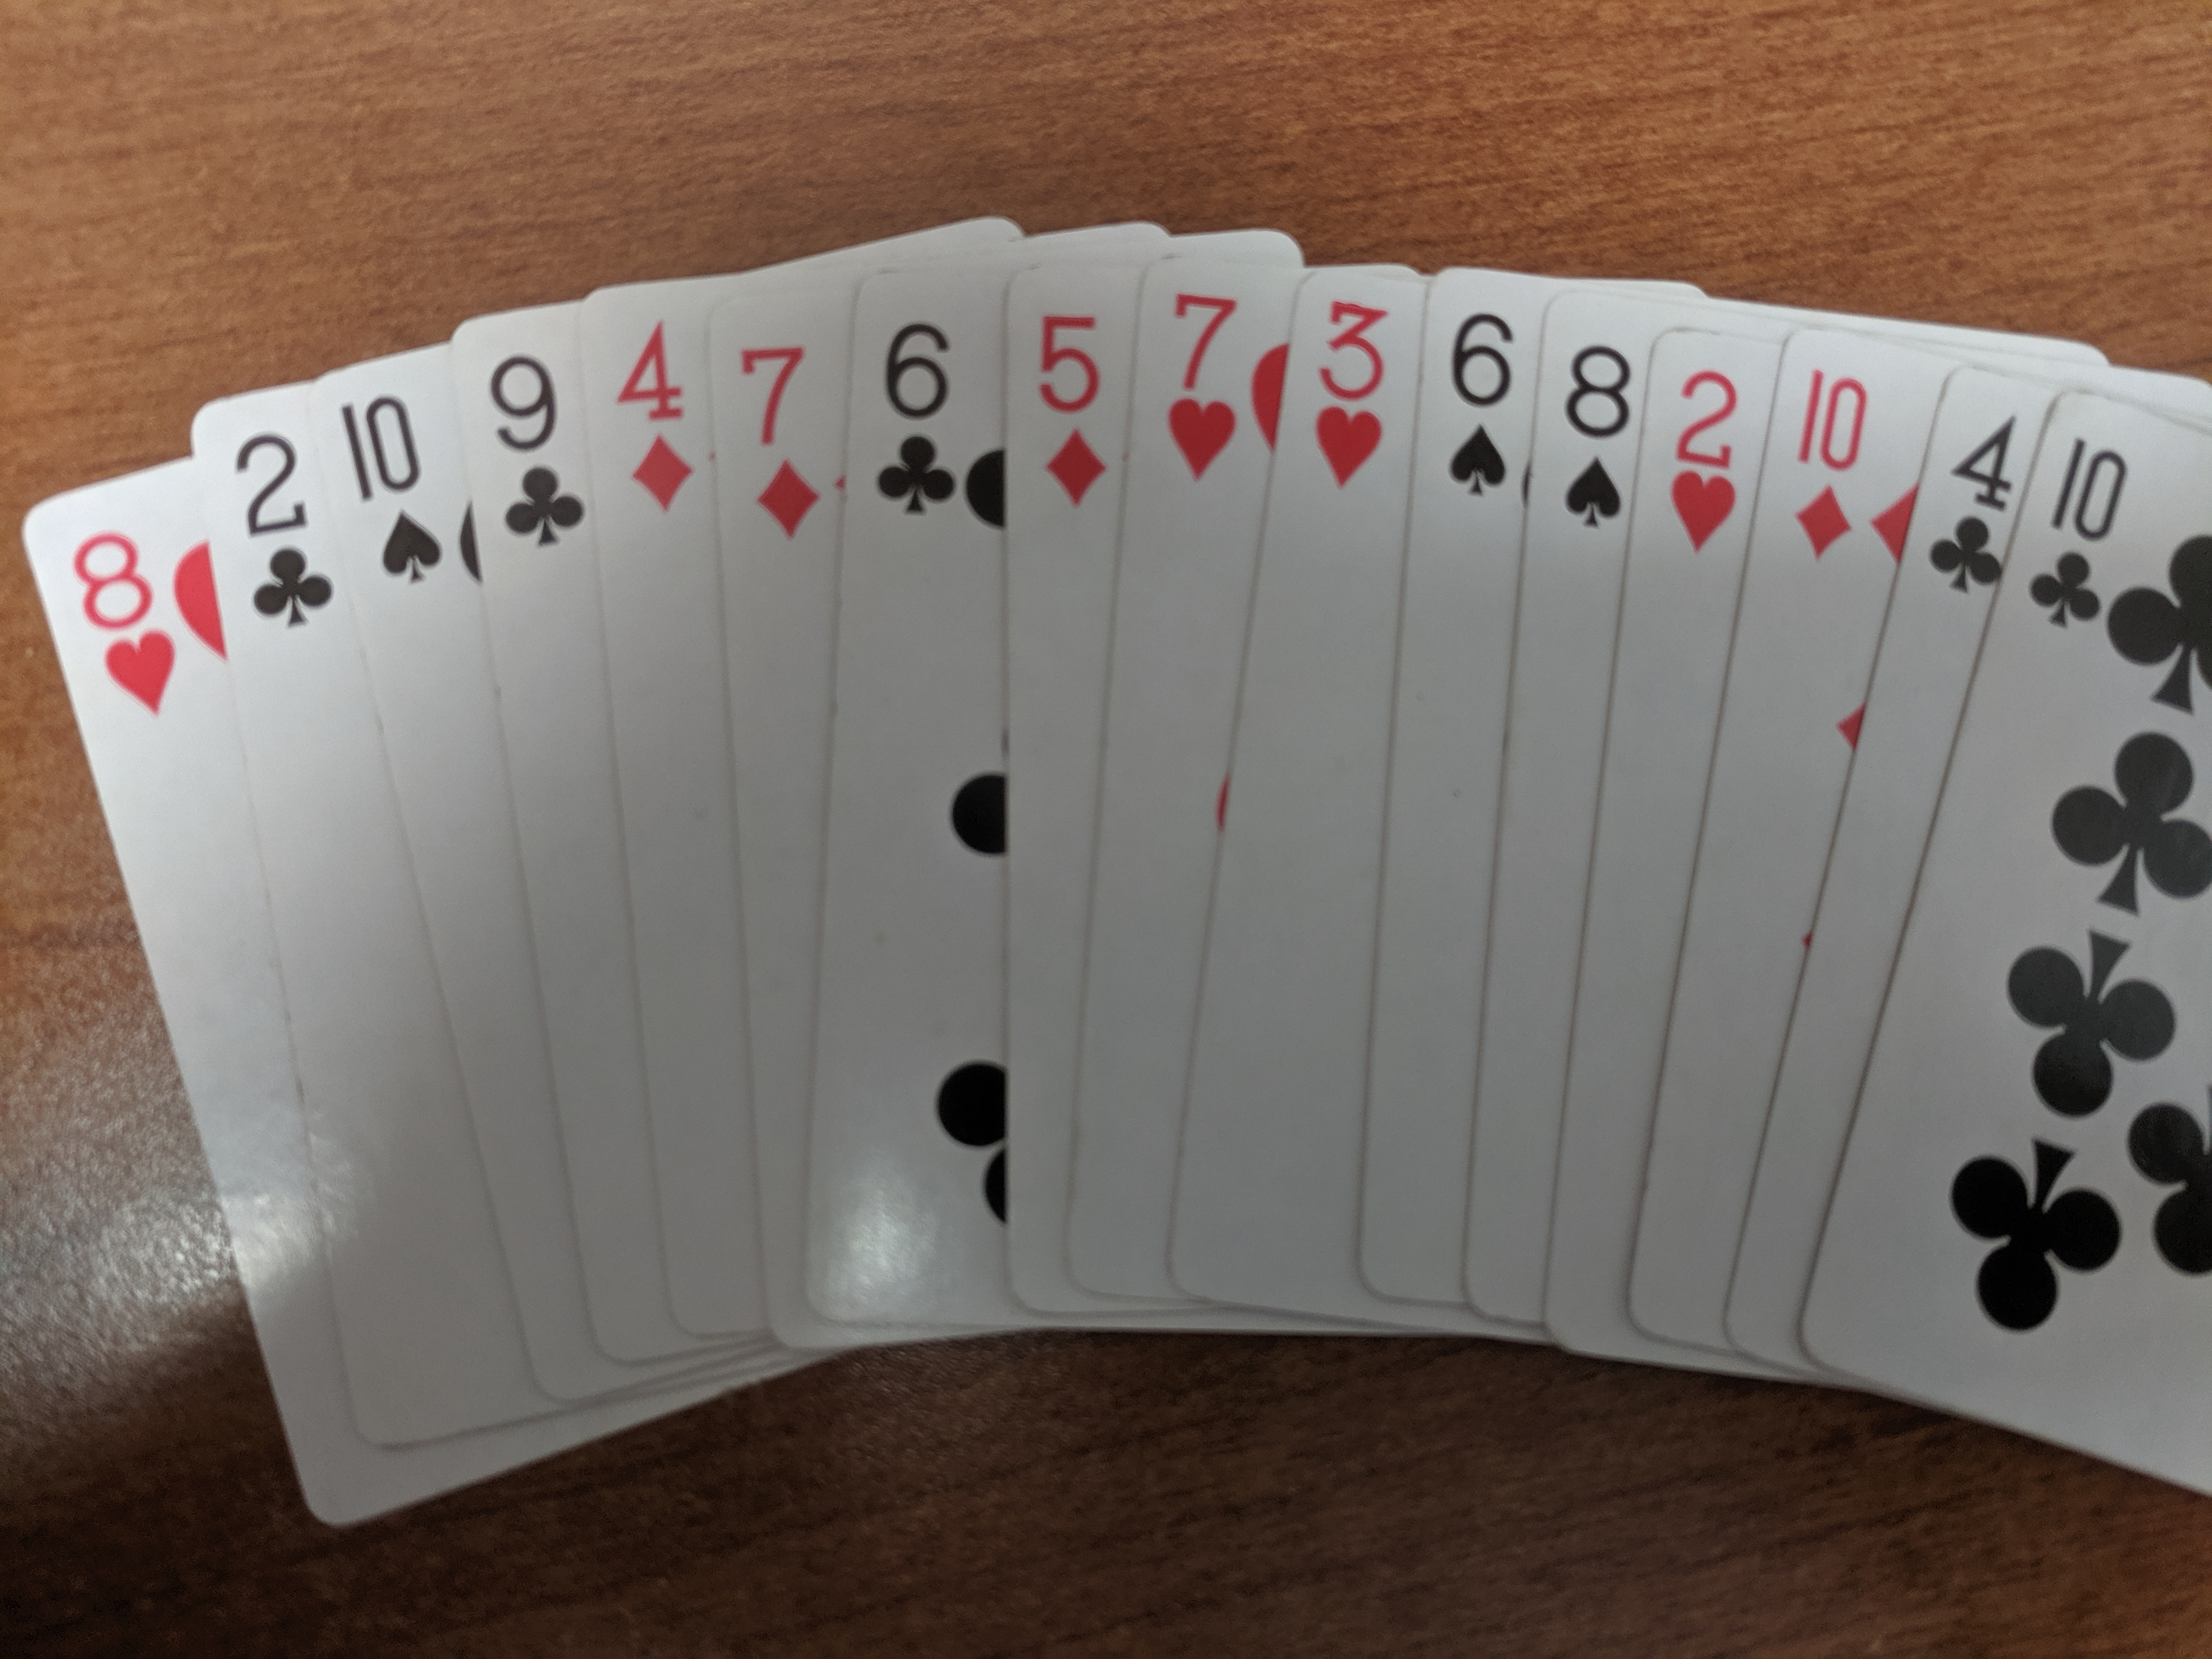
\includegraphics[width=0.5\linewidth]{assets/cards.jpg}\end{center}
